\section{Operationelle Semantik}

Das Folgende bezieht sich auf die \texttt{while}-Sprache (siehe \secref{section:while}).

\begin{definition}
    $\AExp, \BExp, \SExp$: Mengen aller gültigen Ableitungen aus $A$, $B$ bzw. $S$ als Syntaxbaum. Der Ausdruck \texttt{5+7-2*8} lässt sich aus $A$ ableiten. Der entsprechende Syntaxbaum (siehe \figref{fig:syntaxbaum}) ist dann Teil von $\AExp$.
    \[
    a \in \AExp
    \]
    Mengen wie $\AExp$ bezeichnen wir als \textbf{syntaktische Kategorien}.

    \textbf{Zahl} ist eine ganze Zahl aus $\mathbb{Z}$. Die zugehörige syntaktische Kategorie $\Num$. Num ist die Menge aller Zeichenkette, die ganze Zahlen darstellen.
    \begin{align*}
        \texttt{1234} & \in \Num \\
        1234 & \in \mathbb{Z}
    \end{align*}
    Beachte, dass eigentlich der Syntaxbaum von \texttt{1234} gemeint ist

    $\Var$ sind Variablen, die nach Belieben vorhanden sind. Es sind abzählbar unendlich viele.
\end{definition}

% https://dreampuf.github.io/GraphvizOnline/
% digraph G {
%     ordering="out";
%     mult[label="*"];
%     minus[label="-"];
%     plus[label="+"];
%     zahl1[label="Zahl"]; zahl2[label="Zahl"]; zahl3[label="Zahl"]; zahl4[label="Zahl"];
%     minus -> plus -> zahl1 -> 5;
%              plus -> zahl2 -> 7;
%     minus -> mult -> zahl3 -> 2;
%              mult -> zahl4 -> 8;
% }
\begin{figure}[H]
    \centering
    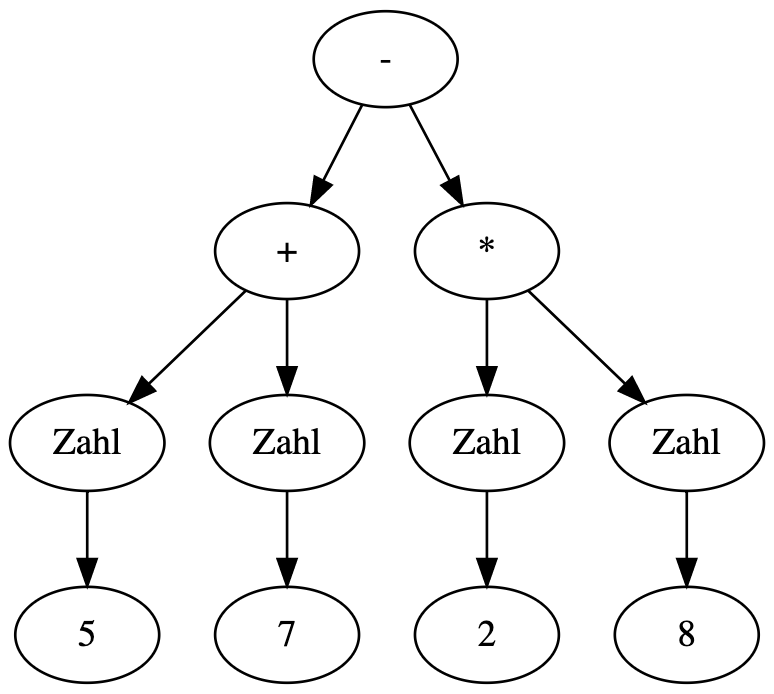
\includegraphics[width=.4\textwidth]{syntaxbaum.png}
    \caption{\texttt{5+7-2*8} $\in \AExp$ als verkürzt dargestellter Syntaxbaum}
    \label{fig:syntaxbaum}
\end{figure}

\begin{remark}
    Unterbäume können auch Elemente einer anderen Kategorie sein.
    % B -> (A < A) \in BExp
    % Unterbaum A \in AExp
\end{remark}

\begin{example}
    Division mit Rest
    \begin{itemize}
        \item Eingabe: $a, b > 0$
        \item Ausgabe: $m ,r \geq 0$, $r < b$, $a = m \cdot b + r$
    \end{itemize}
\end{example}

\begin{lstlisting}[language=C, caption=Division mit Rest]
m := 0;
while b <= a do (
    m := m + 1;
    a := a - b
)
r := a
\end{lstlisting}

Die \emph{Semantik} in \texttt{while} wird gegeben durch eine \emph{semantische Funktion}, eine für jede \emph{syntaktische Kategorie}.

Sei $State = \{ \sigma \,\vert\, \sigma: \Var \to \mathbb{Z} \}$, \zb
\begin{align*}
    \mathcal{N} : \Num & \to \mathbb{Z} \\
    \mathcal{N}\lsem\texttt{-123}\rsem & = -123
\end{align*}

\begin{align*}
    \A: \underbrace{\AExp}_{\text{``Compiler''}} & \to \underbrace{(\State \to \mathbb{Z})}_{\text{``Interpreter''}} \\
    \A\lsem\texttt{x+x*5}\rsem & = (\sigma \mapsto 6 \cdot \sigma(x)) \quad (\text{da }\texttt{x+x*5} = \texttt{6*x})
\end{align*}

\begin{align*}
    \B : \BExp \to (\State \to \{ w, f \}) \\
    \B\lsem\texttt{x<=10}\rsem = \bigg( \sigma \mapsto \begin{cases}
        w & \sigma(x) \leq 10 \\
        f & \sigma(x) > 10
    \end{cases} \bigg)
\end{align*}

\[
S: \SExp \to (\State + \State)
\]

\textbf{Jetzt:} Definition von $\A$ durch Induktion über die Struktur des Syntaxbaums. Die Definition von $\N$ und $\B$ ist eine Übung.

\textbf{Später:} Definition von $S$.



\subsection{Semantik arithmetischer Ausdrücke}

\begin{definition}[Induktive Definition von $\A$]\label{def:Asem}
    Sei $n \in \Num, x \in \Var, \sigma \in \State$ und $a_1, a_2 \in \AExp$. Wir definieren:
    \begin{enumerate}
        \item[(i)] $\A\lsem n \rsem(\sigma) = \N\lsem n \rsem$ \quad\quad (konstante Funktion)
        \item[(ii)] $\A\lsem x \rsem(\sigma) = \sigma(x)$ \quad\quad\quad alternativ: $\A\lsem n \rsem = (\sigma \mapsto \sigma(n))$
        \item[(iii)] $\A\lsem a_1 + a_2 \rsem(\sigma) = \A\lsem a_1 \rsem(\sigma) + \A\lsem a_2 \rsem(\sigma)$ \\[4pt]
        \emph{Bemerkung.} In anderen Sprachen könnte der Aufruf des ersten Summanden Seiteneffekte haben, \dh{} ggf.\ muss man an dieser Stelle aufpassen. In diesem Fall würde der potentenziell veränderte Zustand mit zurückgegeben werden.
        \item[(iv)] Analog für Subtraktion
        \item[(v)] Analog für Multiplikation
    \end{enumerate}
\end{definition}

\begin{remark}
    Für die Definition von semantischen Funktionen fordern wir \textbf{Zusammengesetztheit}, \dh{} in der induktiven Definition darf nur auf Bestandteile des Ausdrucks/Syntaxbaums zugegriffen werden.
\end{remark}

\begin{example}
    Führe Negation ein: $\A \to \dots | -A$.

    Erlaubt ist $\A\lsem -a_1 \rsem(\sigma) = 0 - \A\lsem a_1 \rsem(\sigma)$ aber nicht $\A\lsem -a_1 \rsem(\sigma) = \A\lsem 0 - a_1 \rsem(\sigma)$, da der Ausdruck hier um eine Null erweitert wurde.
\end{example}



%%%%%%%%%%%%%%%%%%%%%%%%%%%%%%%%%%%%%%%%%%%%%%%%%%%%%%%%%%%%%%%%%%%%%
\newpage
\hfill 13.05.
%%%%%%%%%%%%%%%%%%%%%%%%%%%%%%%%%%%%%%%%%%%%%%%%%%%%%%%%%%%%%%%%%%%%%

\begin{theorem}
    $\A$ besitzt die folgenden Eigenschaften:
    \begin{enumerate}
        \item für alle $a \in \AExp$, für alle $\sigma \in \State$ existiert genau eine Zahl $n \in \mathbb{Z}$, sodass $\A\lsem a \rsem (\sigma) = n$. (Voraussetzung: $\sigma$ ist eine totale Funktion.)
        \item $\A$ ist eine totale Funktion.
    \end{enumerate}
\end{theorem}

\begin{proof}[Beweis]
    Skizze:
    \begin{enumerate}
        \item[(b)] folgt aus (a)
        \item[(a)] wird bewiesen durch strukturelle Induktion nach $a$.
    \end{enumerate}
\end{proof}

\par\bigskip
\textbf{Nächste Schritte:}
\begin{enumerate}
    \item[(i)] Der Wert eines Ausdrucks hängt \emph{nur} von den Variables ab, die in ihm vorkommen. (\secref{section:freeVars})
    \item[(ii)] Was passiert in einem arithmetischen Ausdruck, wenn wir eine Variable durch einen Ausdruck ersetzen ($\leadsto$ \emph{Substitution})? (\secref{section:substitution})
\end{enumerate}



% FREIE VARIABLEN %%%%%%%%%%%%%%%%%%%%%%%%%%%%%%%%%%%%%%%%%%%%%%%%%%%%%%%%%%%%%%%%%%%%%%%%%%%
\subsection{Freie Variablen} \label{section:freeVars}

\begin{definition}[Freie Variablen]
    Sei $a \in \AExp$. $\FV(a)$ (``freie Variablen'') ist die Menge aller Variablen, die in $a$ vorkommen. Formal ist das induktiv definiert:
    \begin{enumerate}
        \item $\FV(n) = \emptyset$ \quad\quad\quad (falls $a = n$ (Zahl))
        \item $\FV(x) = \{ x \}$ \quad\quad (falls $a = x$ (Variable))
        \item $\FV(a_1 \;\square\; a_2) = \FV(a_1) \cup \FV(a_2)$ \quad\quad für $\square \in \{ +, -, * \}$
    \end{enumerate}

    Gebundene Variable betrachten wir im Kontekt der \texttt{while}-Sprache nicht. in anderen Sprachen können aber lokale Variablen \zb als solche betrachtet werden.
\end{definition}

\begin{lemma}
    Sei $a \in \AExp$, sei $\sigma, \sigma' \in \State$, sodass $\sigma(x) = \sigma'(x)$ für alle $x \ in\FV(a)$ gilt.

    Dann gilt:
    \[
    \A\lsem a \rsem(\sigma) = \A\lsem a \rsem(\sigma')
    \]
\end{lemma}
\begin{proof}[Beweis]
    Durch strukturelle Induktion nach $a$.

    \emph{Induktionsanfang:}
    \begin{enumerate}
        \item $a = n$, $n$ Zahl
            \begin{align*}
                \A\lsem a \rsem(\sigma) & = \A\lsem n \rsem(\sigma) \\
                & \overset{\defrefshort{def:Asem}(i)}{=} \N\lsem n \rsem \\
                \\
                \A\lsem a \rsem(\sigma') & = \A\lsem n \rsem(\sigma') \\
                & = \N\lsem n \rsem
            \end{align*}

        \item $a = x$, $x$ Variable
            \begin{align*}
                \A\lsem a \rsem(\sigma) & = \A\lsem x \rsem(\sigma) \\
                & \overset{\defrefshort{def:Asem}(ii)}{=} \sigma(x) \\
                \\
                \A\lsem a \rsem(\sigma') & = \A\lsem x \rsem(\sigma') \\
                & = \sigma'(x) \\
                \\
                \FV(a) & = \FV(x) = \{ x \}
            \end{align*}
            Nach Annahme ist $\sigma(x) = \sigma'(x)$, da $x \in \FV(a)$. Daher folgt
            \[
            \A\lsem a \rsem(\sigma) = \A\lsem a \rsem(\sigma')
            \]
    \end{enumerate}

    \emph{Induktionsschritt:}

    $a = a_1 \;\square\; a_2$ mit $\square \in \{ +, -, * \}$

    \begin{align*}
        \A\lsem a \rsem(\sigma) & = \A\lsem a_1 \;\square\; a_2 \rsem(\sigma) \\
        & = \A\lsem a_1 \rsem(\sigma) \;\square\; \A\lsem a_2 \rsem(\sigma) \\
        \\
        \A\lsem a \rsem(\sigma') & = \A\lsem a_1 \;\square\; a_2 \rsem(\sigma') \\
        & = \A\lsem a_1 \rsem(\sigma') \;\square\; \A\lsem a_2 \rsem(\sigma') \\
        \\
        \FV(a) & = \FV(a_1 \;\square\; a_2) \\
        & = \FV(a_1) \cup \FV(a_2)
    \end{align*}
    Insbesondere gilt, dass $\FV(a_1) \subseteq \FV(a)$ und $\FV(a_2) \subseteq \FV(a)$. Daher folgt:

    Da nach Annahme $\sigma(x) = \sigma(x')$ für alle $x \in \FV(a)$, gilt
    \[
    \sigma(x) = \sigma'(x) \text{ für alle } x \in \FV(a_1)
    \]
    und
    \[
    \sigma(x) = \sigma'(x) \text{ für alle } x \in \FV(a_2)
    \]

    Also gelten nach Induktionsvoraussetzung
    \[
    \A\lsem a_1 \rsem(\sigma) = \A\lsem a_1 \rsem(\sigma') \wedge \A\lsem a_2 \rsem(\sigma) = \A\lsem a_2 \rsem(\sigma')
    \]

    Daher folgt:
    \[
    \A\lsem a_1 \rsem(\sigma) \;\square\; \A\lsem a_2 \rsem(\sigma) = \A\lsem a_1 \rsem(\sigma') \;\square\; \A\lsem a_2 \rsem(\sigma')
    \]
\end{proof}



% SUBSTITUTION %%%%%%%%%%%%%%%%%%%%%%%%%%%%%%%%%%%%%%%%%%%%%%%%%%%%%%%%%%%%%%%%%%%%%%%%%%%%%%%%
\subsection{Substitution}\label{section:substitution}

\begin{definition}[Substitution für Ausdrücke] \label{def:substitutionExp}
    Seien $a, a_0 \in \AExp, \, y \in \Var$. Wir definieren $a[y \mapsto a_0]$ als den arithmetischen Ausdruck, in dem jedes Vorkommen von $y$ in $a$ durch $a_0$ ersetzt wird.

    Formal:
    \begin{enumerate}
        \item[(i)] $n[y \mapsto a_0] = n$
        \item[(ii)] $x[y \mapsto a_0] = \begin{cases} a_0 & \text{falls } x = y \\ x & \text{sonst} \end{cases}$
        \item[(iii)] $(a_1 \;\square\; a_2)[y \mapsto a_0] = a_1[y \mapsto a_0] \;\square\; a_2[y \mapsto a_0]$ \quad\quad für $\square \in \{ +, -, * \}$
    \end{enumerate}
\end{definition}

\begin{example}
    \begin{align*}
        a & = \texttt{x + y*2 - z(x + y)} \\
        \texttt{y} & \mapsto \texttt{4*t + 5} \\
        \\
        a[\texttt{y} \mapsto \texttt{4*t + 5}] & = \texttt{x + (4*t + 5)*2 - z(x + (4*t + 5))}
    \end{align*}
    Es werden die Blätter am Syntaxbaum ersetzt, woraus implizit die Präzedenz klar ist (wodurch die obigen Klammern entstehen).

    Ersetzungen dürfen die zu ersetzende Variable enthalten. Da nur einmal ersetzt wird, ist das in Ordnung.
\end{example}

\begin{definition}[Substitution für Zustände]\label{def:substitutionState}
    Sei $\sigma \in \State, \, x \in \Var, \, n \in \mathbb{Z}$. Dann ist $\sigma[x \mapsto n] \in \State$ der Zustand, der wie folgt definiert ist:
    \begin{align*}
        \sigma[x \mapsto n](z) = \begin{cases}
            n & \text{falls } z = x \\
            \sigma(z) & \text{sonst}
        \end{cases}
    \end{align*}
\end{definition}

\begin{lemma}
    Sei $a, a_0 \in \AExp, \, y \in \Var, \, \sigma \in \State$. Dann gilt:
    \begin{align*}
        \A\lsem a[y \mapsto a_0] \rsem(\sigma) & = \A\lsem a \rsem \Big( \sigma\big[y \mapsto \A\lsem a_0 \rsem(\sigma)\big] \Big)
    \end{align*}
\end{lemma}

Das Lemma setzt Semantik und Syntax in Verbindung: Wir können syntaktisch Variable durch Teilausdrücke ersetzen und das ist äquivalent dazu, erst den Teilausdruck auszuwerten und mit diesen Wert im Zustand den ursprünglichen Ausdruck auszuwerten.

\begin{example}
    \begin{align*}
    a & = x + y \\
    a_0 & = x * y \\
    \sigma: & \; [x \mapsto 2; y \mapsto 10] \\
    \\
    (x + (x * y))[x \mapsto 2; y \mapsto 10] \quad & \square\; (x + y)[x \mapsto 2; y \mapsto 20] \\
    2 + (2 * 10) \quad & \square\; 2 + 20 \\
    22 \quad & = 22
\end{align*}
\end{example}


\begin{proof}[Beweis]
    Durch strukturelle Induktion nach $a$ (nicht $a_0$!).

    \emph{Induktionsanfang:}
    \begin{enumerate}
        \item $a = n$, $n$ Zahl
            \begin{align*}
                \A\lsem a[y \mapsto a_0] \rsem(\sigma) & = \A\lsem n[y \mapsto a_0] \rsem(\sigma) \\
                & \overset{\defrefshort{def:substitutionExp}(i)}{=} \A\lsem n \rsem(\sigma) \\
                & = n \\
                \\
                \A\lsem n \rsem(\sigma[y \mapsto \A\lsem a_0 \rsem(\sigma)]) & = n \quad\quad \text{(rechte Seite)}
            \end{align*}

        \item $a = x$, $x$ Variable
            \begin{align*}
                \A\lsem x[y \mapsto a_0] \rsem(\sigma) & \overset{\defrefshort{def:substitutionExp}(iii)}{=} \begin{cases}
                    \A\lsem a_0 \rsem(\sigma) & \text{falls } x = y \\
                    \A\lsem x \rsem(\sigma) = \sigma(x) & \text{sonst}
                \end{cases} \\
                \\
                \A\lsem x \rsem(\sigma[y \mapsto \A\lsem a_0 \rsem(\sigma)]) & \overset{\defrefshort{def:substitutionState}}{=} (\sigma[y \mapsto \A\lsem a_0 \rsem(\sigma)])(x) \quad\quad \text{(rechte Seite)} \\
                & = \begin{cases}
                    \A\lsem a_0 \rsem(\sigma) & \text{falls } x = y \\
                    \sigma(x) & \text{sonst}
                \end{cases}
            \end{align*}
    \end{enumerate}

    \emph{Induktionsschritt:} Straight forward.
\end{proof}